\documentclass{article}
% main document, called main.tex
\usepackage{tikz}
\usepackage{tkz-graph}
\usetikzlibrary{external}
\tikzexternalize
% activate!
%\tikzset{ EdgeStyle/.append style = {->, bend left} }
%  LabelStyle/.style = { rectangle, rounded corners, draw,
%    minimum width = 2em, fill = yellow!50,
%  text = red, font = \bfseries },
%  VertexStyle/.append style = { inner sep=5pt,
%  font = \Large\bfseries},
\begin{document}
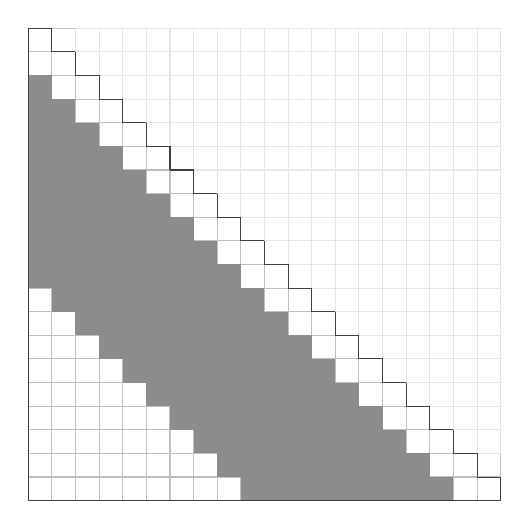
\begin{tikzpicture}
  \foreach \y in {0,0.3,...,6.0} {
      \foreach \x in {0,0.3,...,6.0} {
      \pgfmathsetmacro{\sumxy}{\x+\y};
          \ifthenelse{\lengthtest{\sumxy pt>6.1pt}}{
            \draw[draw=black!10, fill=white] (\x,\y) rectangle ++(0.3,0.3); 
          } {
              \draw[draw=black!25, fill=white] (\x,\y) rectangle ++(0.3,0.3); 
          }
      }
  }
  %
  \foreach \x in {0.0,0.3,...,6.0} {
      \foreach \y in {0.0,0.3,...,6.0} {
      \pgfmathsetmacro{\sumxy}{\x+\y};
          \ifthenelse{\lengthtest{\sumxy pt>5.2pt} \OR \lengthtest{\sumxy pt < 2.5 pt}}{
          } {
              \draw[draw opacity=0, fill=black!45] (\x,\y) rectangle ++(0.3,0.3); 
          }
      }
  }
  %
  \draw[draw=black!75] (0,0) -- (6,0);
  \draw[draw=black!75] (0,0) -- (0,6);
  \foreach \x in {0.3,0.6,...,6.3} {
    \draw[draw=black!75] (\x,6.3-\x) -- (\x,6.0-\x);
    \draw[draw=black!75] (\x,6.3-\x) -- (\x-0.3,6.3-\x);
  }
\end{tikzpicture}

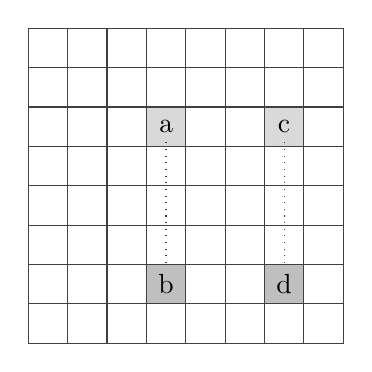
\begin{tikzpicture}
  %\draw[draw=black!75, fill=white] (\x,\y) rectangle ++(0.5,0.5); 
  \fill[color=black!15] (1.5,2.5) +(-.25,-.25) rectangle ++(.25,.25); 
  \draw (1.5,2.5) node (a) {a};
  \fill[color=black!15] (3.0,2.5) +(-.25,-.25) rectangle ++(.25,.25); 
  \draw (3.0,2.5) node (c) {c};
  \fill[color=black!25] (1.5,0.5) +(-.25,-.25) rectangle ++(.25,.25); 
  \draw (1.5,0.5) node (b) {b};
  \fill[color=black!25] (3.0,0.5) +(-.25,-.25) rectangle ++(.25,.25); 
  \draw (3.0,0.5) node (d) {d};
  
  \foreach \y in {0,0.5,...,3.5} {
      \foreach \x in {0,0.5,...,3.5} {
        \draw[draw=black!75, fill=white, fill opacity=0.0] (\x,\y) +(-.25,-.25) rectangle ++(.25,.25); 
      }
  }
  \draw[draw=black!75,dotted] (a) -- (b);
  \draw[draw=black!75,dotted] (c) -- (d);
\end{tikzpicture}
\end{document}
